\label{chap:capitulo1}
 


\section{Capítulo 1: Caracterización del caso de estudio en Industria 4.0}
\label{cap:caso_estudio}

Este capítulo caracteriza el caso de estudio que sirve de base al presente trabajo, inspirado en un proyecto de integración IIoT desarrollado por la empresa aliada DAUTOM S.A.S. en el sector molinero. A continuación se describe el contexto del proyecto, el proceso productivo y su flujo operacional.

\subsection{Contexto del caso de estudio}

El caso de estudio parte de un proyecto real de integración IIoT desarrollado por \href{https://www.dautom.com.co/}{DAUTOM S.A.S.} en Barranquilla, Colombia. El proyecto conectó las áreas de empaque de harina de maíz y de trigo a una plataforma MES (Manufacturing Execution System), donde la información recolectada se emplea para calcular rendimientos de proceso, evaluar la disponibilidad de las máquinas y controlar la calidad del producto.

\subsection{Proceso y flujo operacional del área de empaque}

Esta área toma la harina producida en los molinos y la envasa para su comercialización. Al ser el punto final de la cadena antes de la distribución al cliente, se convierte en un nodo crítico de medición: cualquier pérdida de disponibilidad o calidad se traduce directamente en producto no despachado.

Cada área de empaque —trigo y maíz— opera con dos líneas de producción independientes, identificadas como Línea A y Línea B. El flujo fisico del producto inicia una vez el material sale de los molinos y llega a silos de almacenamiento temporal; a partir de ahí, cada línea ejecuta los siguientes pasos:

\begin{enumerate}
    \item \textbf{Empacado:} el producto se traslada mediante sistemas de transporte neumático y mecánico hacia las máquinas encargadas de envasar la harina en bolsas de una libra o de un kilo. Cada línea dispone de \textbf{2 empacadoras} (cuatro por área), lo que permite mantener la continuidad operativa ante mantenimientos o fallas en una de ellas.
    
    \item \textbf{Enfardado:} las bolsas se agrupan y embalan en fardos mediante la enfardadora, equipo que facilita el manejo, almacenamiento y transporte del producto. Cada línea cuenta con \textbf{1 enfardadora} (dos por área). La cantidad de bolsas del fardo depende de la presentación: para libra, cada fardo contiene 24 unidades; para kilo, 20 unidades.
\end{enumerate}

Este proceso se ejecuta siempre dentro del contexto de una orden de producción (\textit{Work Order}, WO): un registro creado en el MES sobre la plataforma Ignition, a nivel de línea, que especifica el producto a envasar (harina de trigo o de maíz), la presentación (libra o kilo) y la cantidad meta de unidades. La ejecución de una WO, con sus tiempos reales de inicio y fin, se denomina \textit{corrida}. Una vez inicia la corrida, el sistema vincula automáticamente los datos capturados en planta con la WO correspondiente, y registra en tiempo real los eventos del ciclo productivo: inicio, pausas, reanudaciones y cierre. Esta vinculación entre los datos operativos y el contexto de negocio de cada corrida es lo que permite, más adelante, calcular indicadores como el cumplimiento de la orden o la eficiencia de línea, y es también uno de los elementos que la herramienta LLM deberá interpretar para responder consultas que combinen información en tiempo real con el estado de la producción planificada.

    La figura \ref{fig:flujo_empaque} muestra esquema que representa el flujo operativo descrito anteriormente. 
    
    \begin{figure}[H]
        \centering
        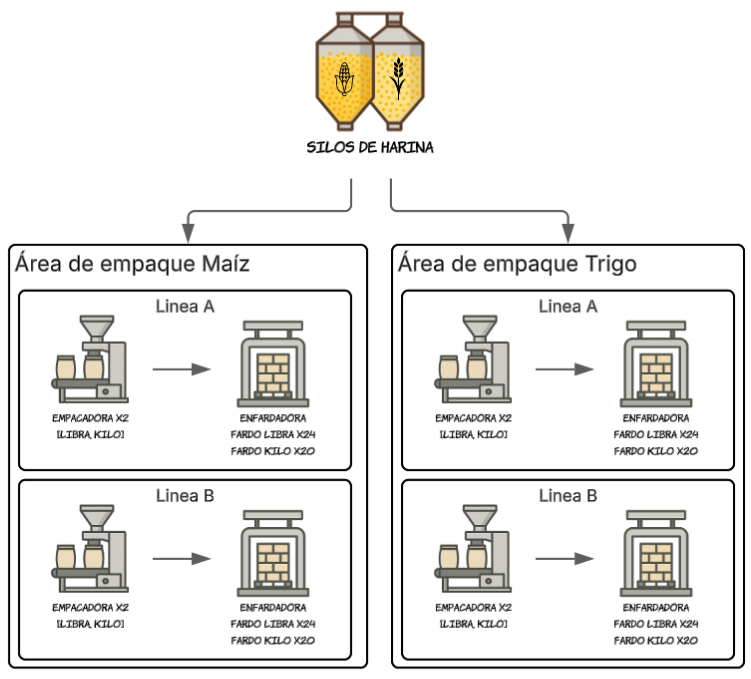
\includegraphics[width=1\textwidth]{Figuras/FlujoMolineria.png}
        \caption{Esquema del flujo operativo del caso de estudio.}
        \label{fig:flujo_empaque}
    \end{figure}

\subsection{Adquisición de datos}

La infraestructura de adquisición de datos de las áreas de empaque se basa en una arquitectura distribuida de controladores industriales que capturan información operativa en tiempo real y la transmiten hacia el centro de control. La Figura \ref{fig:arquitectura_iiot} ilustra esta arquitectura IIoT para las dos áreas del caso de estudio.

\begin{figure}[H]
    \centering
    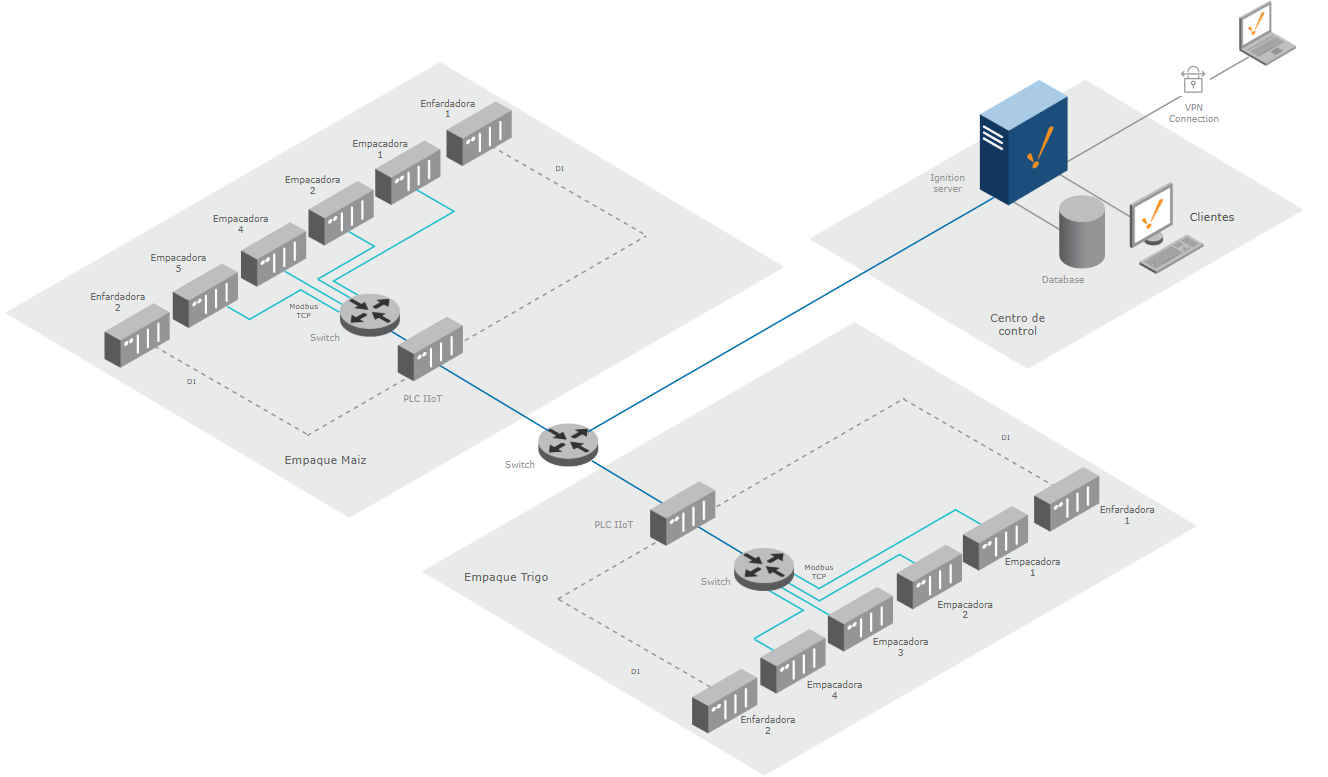
\includegraphics[width=1\textwidth]{Figuras/diagrama_arquitectura.png}
    \caption{Arquitectura IIoT del caso de estudio \textcolor{red}{Falta actualizar esta figura}.}
    \label{fig:arquitectura_iiot}
\end{figure}

\subsubsection{Datos capturados en planta}

\begin{enumerate}
    \item \textbf{Empacadoras:} cada una cuenta con un PLC Omron dedicado que gestiona su lógica de control y captura las siguientes variables:
    \begin{itemize}
        \item \textbf{Conteo de bolsas producidas:} contador acumulado de unidades empacadas.
        \item \textbf{Tiempo de ciclo:} tiempo requerido para completar el empaque de una unidad.
        \item \textbf{Estado de la máquina:} marcha, paro, alarma o mantenimiento.
    \end{itemize}
    Como cada línea dispone de dos empacadoras, cada área cuenta con cuatro PLCs Omron.

    \item \textbf{Enfardadoras:} a diferencia de las empacadoras, solo se tiene acceso a sus señales de entrada/salida (I/O), que proporcionan:
    \begin{itemize}
        \item \textbf{Conteo de bolsas entrantes:} señal de pulsos que registra las bolsas que ingresan a la enfardadora.
        \item \textbf{Estado de actividad:} señal digital que indica si está activa o inactiva.
        \item \textbf{Conteo de fardos producidos:} contador de fardos completos generados.
    \end{itemize}
\end{enumerate}

\subsubsection{Transmisión de datos: red de campo y capa Edge}

Dentro de cada área, los PLCs Omron de las empacadoras se comunican mediante \textbf{Modbus TCP} hacia un switch local, que a su vez los conecta a un \textbf{PLC IIoT (Weidmüller)}. Las señales I/O de las enfardadoras, en cambio, se conectan de forma directa a este mismo PLC IIoT, sin pasar por el switch. El PLC IIoT actúa como concentrador de datos (\textit{Data Gateway}) de toda el área, y cumple las siguientes funciones:

\begin{itemize}
    \item Adquiere la información de los cuatro PLCs Omron y las dos enfardadoras.
    \item Normaliza y estructura los datos según un formato estándar.
    \item Realiza \textit{buffering} local para garantizar la entrega confiable ante fallas de red.
    \item Transmite los datos consolidados hacia el centro de control mediante el protocolo \textbf{OPC UA}, a través de un segundo switch que enruta el tráfico de ambas áreas.
\end{itemize}

El protocolo OPC UA se utiliza como medio de comunicación entre los PLCs IIoT y el centro de control gracias a su interoperabilidad entre fabricantes, su seguridad mediante cifrado y autenticación, y su modelado orientado a objetos, que facilita la organización jerárquica de la información.

\subsection{Centro de control}

El centro de control constituye el núcleo de la arquitectura. Sobre él corre la plataforma \textbf{Ignition}, que integra dos componentes fundamentales: una \textbf{base de datos} que almacena la información operacional recibida desde planta, y la aplicación \textbf{MES}, encargada de gestionar la planificación y ejecución de la producción. Juntos, estos componentes reciben, almacenan y ponen a disposición toda la información recolectada en las dos áreas de empaque.

\subsubsection{Ignition Gateway}

\textbf{Ignition Gateway} funciona como servidor central de la arquitectura, alojando tanto la base de datos como la aplicación MES. Sus funciones principales incluyen:

\begin{itemize}
    \item Establecer conexiones OPC UA con los PLCs IIoT de las dos áreas.
    \item Adquirir y procesar en tiempo real todas las variables del proceso, almacenándolas en la base de datos operacional.
    \item Ejecutar la aplicación MES para la gestión integral de las órdenes de producción.
    \item Habilitar el acceso remoto de los clientes mediante conexión VPN, para la consulta de información y reportes.
\end{itemize}

\subsubsection{Aplicación MES}

La aplicación MES implementada sobre Ignition gestiona la planificación y ejecución de la producción a través de las órdenes de producción (WO) y las corridas descritas anteriormente. Entre sus capacidades se incluyen:

\begin{itemize}
    \item Crear y administrar WO para cada línea de producción (Línea A y B, tanto de Trigo como de Maíz), especificando producto, presentación y cantidad meta.
    \item Registrar el inicio de cada corrida sobre una línea específica, así como sus pausas, reanudaciones y cierre.
    \item Vincular los datos de producción capturados en planta (conteo de unidades, tiempos de ciclo, estados de máquina) con la WO y la corrida correspondientes.
\end{itemize}

\subsubsection{Generación de KPIs}

La integración entre el MES y los datos adquiridos en tiempo real habilita el cálculo automático de indicadores clave de desempeño (KPIs), eliminando la captura manual y garantizando que los indicadores se basen en información confiable y actualizada:

\begin{itemize}
    \item \textbf{Disponibilidad:} porcentaje del tiempo de la corrida durante el cual la empacadora estuvo operando, descontando paros no programados y mantenimientos.
    \item \textbf{Rendimiento:} razón entre la velocidad real de producción y la velocidad nominal de la máquina, evaluada frente a la WO activa.
    \item \textbf{Calidad:} porcentaje de unidades producidas que cumplen los estándares de conformidad, sin defectos ni reprocesos.
    \item \textbf{OEE (Overall Equipment Effectiveness):} indicador compuesto que resulta de multiplicar disponibilidad, rendimiento y calidad, ofreciendo una medida integral de la eficiencia del equipo.
\end{itemize}

Esta integración constituye un elemento fundamental de la arquitectura, ya que transforma datos operacionales en información accionable para la toma de decisiones estratégicas y la mejora continua de los procesos productivos.

\subsubsection{Base de datos histórica}

El sistema incorpora una base de datos histórica que almacena series temporales de todas las variables monitorizadas, cumpliendo tres funciones críticas:

\begin{itemize}
    \item \textbf{Análisis retrospectivo:} permite realizar estudios de tendencias, identificación de patrones de producción y evaluación del desempeño histórico de equipos y procesos.
    \item \textbf{Trazabilidad regulatoria:} garantiza el cumplimiento de requisitos normativos relacionados con la trazabilidad de productos y procesos, manteniendo registros auditables de todas las operaciones.
    \item \textbf{Optimización de procesos:} proporciona la base de datos necesaria para aplicaciones de analítica avanzada, aprendizaje automático y modelos predictivos orientados a la optimización continua.
\end{itemize}

La arquitectura de almacenamiento está diseñada para mantener la integridad de los datos a largo plazo, garantizando su disponibilidad para consultas históricas y análisis futuros.

\subsection{Requerimientos y desafíos para la analítica de datos}
\label{requerimientosdesafios}

A continuación se describe en detalle cada requerimiento identificado y los desafíos técnicos asociados a su implementación.

\subsubsection{R1: Interpretación de consultas en lenguaje natural con conocimiento técnico del dominio}

\textbf{Descripción del requerimiento:}

El sistema LLM debe comprender consultas en lenguaje natural que incluyan términos técnicos de manufactura y ser capaz de identificar qué datos del UNS necesita consultar para responder. Esto implica que usuarios sin conocimientos técnicos especializados puedan realizar preguntas sobre el proceso productivo y obtener respuestas precisas y contextualizadas.

\textbf{Desafíos identificados:}

\textit{D1.1 - Ambigüedad en términos técnicos:} Palabras como \textit{disponibilidad}, \textit{rendimiento} o \textit{producción} pueden tener diferentes significados según el contexto en el que se utilicen. Por ejemplo, \textit{disponibilidad} puede referirse a si la máquina está funcionando (uptime) o a si hay material disponible para producir. De manera similar, \textit{rendimiento} puede aludir al rendimiento de una máquina individual (unidades producidas por hora) o al rendimiento global de una línea de producción. El LLM debe entender el contexto de la pregunta para interpretar correctamente el término y acceder a las variables apropiadas del namespace. Esto requiere no solo procesamiento de lenguaje natural, sino también conocimiento del dominio industrial y la semántica de las métricas de manufactura.

\textit{D1.2 - Comprensión de relaciones entre variables:} Preguntas como \textit{¿por qué bajó la producción ayer?} requieren analizar múltiples factores que pueden estar relacionados: paros de máquinas no programados, incremento en tiempos de ciclo, cambios de producto que requieren ajustes, o falta de material en los silos. El LLM debe saber qué variables están relacionadas causalmente y buscar correlaciones entre ellas, no solo reportar un dato aislado. Este desafío implica que el modelo debe tener capacidad de razonamiento sobre las relaciones funcionales entre diferentes componentes del sistema productivo y cómo estas interacciones afectan los KPIs resultantes.

\textit{D1.3 - Mapeo de lenguaje natural a la estructura del namespace:} El usuario puede utilizar referencias ambiguas como \textit{la empacadora de trigo} sin especificar cuál de las 4 empacadoras del área de trigo se está consultando. De manera similar, expresiones como \textit{la línea A} pueden referirse a Línea A de Trigo o Línea A de Maíz. El LLM debe ser capaz de pedir aclaraciones cuando sea necesario (\textit{¿Te refieres a la Línea 1 del área de Trigo o de Maíz?}) o usar el contexto previo de la conversación para resolver la ambigüedad de forma inteligente. Esto requiere mantener estado conversacional y aplicar heurísticas de resolución de referencias.

\subsubsection{R2: Generación de reportes personalizados con análisis comparativos}

\textbf{Descripción del requerimiento:}

La herramienta debe generar reportes que no solo muestren números crudos, sino que incluyan comparaciones útiles (vs. día anterior, vs. otras líneas, vs. meta establecida en la orden de producción) y detecten automáticamente anomalías o patrones relevantes para la toma de decisiones.

\textbf{Desafíos identificados:}

\textit{D2.1 - Identificar qué comparaciones son relevantes:} No todas las comparaciones tienen sentido o aportan valor en el contexto de manufactura. Por ejemplo, comparar la producción de un lunes con un domingo puede ser engañoso si los turnos de fin de semana operan con menor personal o producen referencias diferentes. El LLM debe incorporar lógica operacional para saber qué comparaciones aportan valor en cada contexto. Esto incluye comparaciones con el mismo día de la semana anterior (para eliminar efectos de calendario), comparaciones entre líneas que producen el mismo producto (para identificar ineficiencias relativas), y comparaciones contra las metas establecidas en las órdenes de producción del MES.

\textit{D2.2 - Combinar datos de múltiples fuentes:} Para generar reportes completos y contextualizados, el LLM debe integrar información de tres fuentes principales:

\begin{itemize}
    \item \textbf{UNS:} Datos operacionales en tiempo real (conteos actuales de bolsas, tiempos de ciclo recientes, estados actuales de máquinas, eventos de alarma activos).
    \item \textbf{MES integrado en Ignition:} Información contextual sobre la operación (qué WO está activa, qué producto se está empacando, cantidades meta, tiempos de la corrida).
    \item \textbf{Base de datos histórica:} Datos de producción de días, semanas o meses anteriores que permiten análisis de tendencias, detección de degradación de equipos, y comparaciones temporales.
\end{itemize}

La integración coherente de estas fuentes permite que el LLM genere análisis completos. Por ejemplo: \textit{La producción de hoy está 15\% por debajo del mismo día de la semana pasada (BD histórica), la Línea A de Trigo está trabajando en la WO \#12345 presentación kilo con una meta de 5000 unidades (MES), y actualmente la Empacadora 2 está en estado de alarma desde hace 10 minutos (UNS), lo que explica la desviación observada}. Este desafío requiere que el LLM orqueste consultas a múltiples sistemas, reconcilie diferencias en granularidad temporal entre fuentes, y sintetice la información de forma coherente.

\textit{D2.3 - Adaptar el reporte según el perfil del usuario:} Diferentes stakeholders en la organización tienen necesidades de información distintas:

\begin{itemize}
    \item Un \textbf{gerente de producción} necesita ver KPIs agregados por área, tendencias semanales o mensuales, y comparaciones de eficiencia entre turnos o líneas.
    \item Un \textbf{supervisor de turno} necesita detalles específicos sobre qué ocurrió durante su periodo de responsabilidad, en qué equipos se presentaron problemas, y qué acciones correctivas se tomaron.
    \item Un \textbf{técnico de mantenimiento} necesita información sobre frecuencia de fallas por equipo, tiempos promedio de reparación, y patrones de degradación que sugieran mantenimientos preventivos.
\end{itemize}

El sistema debe ser capaz de ajustar automáticamente el contenido, nivel de detalle, métricas presentadas y formato de salida según el perfil del usuario que realiza la consulta. Esto implica implementar perfiles de usuario con permisos y preferencias diferenciadas.

\subsubsection{R3: Acceso eficiente a datos históricos y en tiempo real}

\textbf{Descripción del requerimiento:}

El sistema debe poder consultar tanto los datos en tiempo real disponibles en el UNS como el histórico almacenado en bases de datos relacionales, y combinarlos de forma coherente para responder consultas que abarquen diferentes periodos de tiempo, desde minutos recientes hasta meses o años anteriores.

\textbf{Desafíos identificados:}

\textit{D3.1 - Generar consultas eficientes a la base de datos:} El LLM debe traducir preguntas en lenguaje natural a consultas de base de datos (SQL) que sean eficientes y no generen carga computacional excesiva. Por ejemplo, si el usuario pregunta \textit{¿cuál fue el promedio de producción del último mes?}, el LLM debe generar una query que utilice tablas agregadas pre-calculadas o índices apropiados, en lugar de escanear millones de registros individuales. Esto requiere que el LLM tenga conocimiento de:
\begin{itemize}
    \item El esquema de la base de datos (tablas, columnas, relaciones)
    \item Los índices disponibles y cómo aprovecharlos
    \item Estrategias de agregación eficiente (uso de tablas materializadas, vistas agregadas)
    \item Limitaciones de rendimiento del sistema de base de datos
\end{itemize}

La generación de queries SQL eficientes es crítica para garantizar tiempos de respuesta aceptables, especialmente cuando se consultan periodos extensos con alta densidad de datos.

\textit{D3.2 - Seleccionar la granularidad adecuada de los datos:} Los datos industriales se almacenan con diferentes frecuencias de muestreo dependiendo de la variable y el propósito. Para periodos cortos de tiempo (última hora, último turno) es apropiado usar datos de alta frecuencia que capturan cada evento significativo. Sin embargo, para periodos largos (último mes, último trimestre) es más eficiente usar agregaciones por hora, por turno, o por día. El LLM debe decidir automáticamente qué nivel de detalle (granularidad) usar según el rango temporal que especifica el usuario en su consulta. Por ejemplo:
\begin{itemize}
    \item "Producción en los últimos 30 minutos" → datos con granularidad de minutos
    \item "Producción del día de ayer" → datos agregados por hora
    \item "Producción del último mes" → datos agregados por día o por turno
\end{itemize}

Esta selección automática de granularidad balancea la precisión de la respuesta con la eficiencia computacional, evitando procesar datos innecesariamente detallados cuando no aportan valor adicional a la consulta.

\subsubsection{Síntesis de requerimientos y desafíos}

Los tres requerimientos identificados y sus desafíos asociados representan los aspectos técnicos críticos que debe abordar la integración de una herramienta LLM con la arquitectura UNS del caso de estudio. El Requerimiento 1 se enfoca en las capacidades de comprensión del lenguaje natural y mapeo al dominio industrial. El Requerimiento 2 aborda la generación inteligente de insights y la personalización de reportes. El Requerimiento 3 trata los aspectos de arquitectura de datos y eficiencia en el acceso a información histórica y en tiempo real.

Estos requerimientos guiarán el diseño de la solución propuesta en los capítulos subsiguientes y servirán como base para la definición de métricas de validación del sistema integrado.